%<dscrpt>Fichier de déclarations Latex à inclure au début d'un élément de cours.</dscrpt>

\documentclass[a4paper]{article}
\usepackage[hmargin={1.8cm,1.8cm},vmargin={2.4cm,2.4cm},headheight=13.1pt]{geometry}

%includeheadfoot,scale=1.1,centering,hoffset=-0.5cm,
\usepackage[pdftex]{graphicx,color}
\usepackage[french]{babel}
%\selectlanguage{french}
\addto\captionsfrench{
  \def\contentsname{Plan}
}
\usepackage{fancyhdr}
\usepackage{floatflt}
\usepackage{amsmath}
\usepackage{amssymb}
\usepackage{amsthm}
\usepackage{stmaryrd}
%\usepackage{ucs}
\usepackage[utf8]{inputenc}
%\usepackage[latin1]{inputenc}
\usepackage[T1]{fontenc}


\usepackage{titletoc}
%\contentsmargin{2.55em}
\dottedcontents{section}[2.5em]{}{1.8em}{1pc}
\dottedcontents{subsection}[3.5em]{}{1.2em}{1pc}
\dottedcontents{subsubsection}[5em]{}{1em}{1pc}

\usepackage[pdftex,colorlinks={true},urlcolor={blue},pdfauthor={remy Nicolai},bookmarks={true}]{hyperref}
\usepackage{makeidx}

\usepackage{multicol}
\usepackage{multirow}
\usepackage{wrapfig}
\usepackage{array}
\usepackage{subfig}


%\usepackage{tikz}
%\usetikzlibrary{calc, shapes, backgrounds}
%pour la présentation du pseudo-code
% !!!!!!!!!!!!!!      le package n'est pas présent sur le serveur sous fedora 16 !!!!!!!!!!!!!!!!!!!!!!!!
%\usepackage[french,ruled,vlined]{algorithm2e}

%pr{\'e}sentation du compteur de niveau 2 dans les listes
\makeatletter
\renewcommand{\labelenumii}{\theenumii.}
\renewcommand{\thesection}{\Roman{section}.}
\renewcommand{\thesubsection}{\arabic{subsection}.}
\renewcommand{\thesubsubsection}{\arabic{subsubsection}.}
\makeatother


%dimension des pages, en-t{\^e}te et bas de page
%\pdfpagewidth=20cm
%\pdfpageheight=14cm
%   \setlength{\oddsidemargin}{-2cm}
%   \setlength{\voffset}{-1.5cm}
%   \setlength{\textheight}{12cm}
%   \setlength{\textwidth}{25.2cm}
   \columnsep=1cm
   \columnseprule=0.5pt

%En tete et pied de page
\pagestyle{fancy}
\lhead{MPSI-\'Eléments de cours}
\rhead{\today}
%\rhead{25/11/05}
\lfoot{\tiny{Cette création est mise à disposition selon le Contrat\\ Paternité-Pas d'utilisations commerciale-Partage des Conditions Initiales à l'Identique 2.0 France\\ disponible en ligne http://creativecommons.org/licenses/by-nc-sa/2.0/fr/
} }
\rfoot{\tiny{Rémy Nicolai \jobname}}


\newcommand{\baseurl}{http://back.maquisdoc.net/data/cours\_nicolair/}
\newcommand{\urlexo}{http://back.maquisdoc.net/data/exos_nicolair/}
\newcommand{\urlcours}{https://maquisdoc-math.fra1.digitaloceanspaces.com/}

\newcommand{\N}{\mathbb{N}}
\newcommand{\Z}{\mathbb{Z}}
\newcommand{\C}{\mathbb{C}}
\newcommand{\R}{\mathbb{R}}
\newcommand{\D}{\mathbb{D}}
\newcommand{\K}{\mathbf{K}}
\newcommand{\Q}{\mathbb{Q}}
\newcommand{\F}{\mathbf{F}}
\newcommand{\U}{\mathbb{U}}
\newcommand{\p}{\mathbb{P}}


\newcommand{\card}{\mathop{\mathrm{Card}}}
\newcommand{\Id}{\mathop{\mathrm{Id}}}
\newcommand{\Ker}{\mathop{\mathrm{Ker}}}
\newcommand{\Vect}{\mathop{\mathrm{Vect}}}
\newcommand{\cotg}{\mathop{\mathrm{cotan}}}
\newcommand{\sh}{\mathop{\mathrm{sh}}}
\newcommand{\ch}{\mathop{\mathrm{ch}}}
\newcommand{\argsh}{\mathop{\mathrm{argsh}}}
\newcommand{\argch}{\mathop{\mathrm{argch}}}
\newcommand{\tr}{\mathop{\mathrm{tr}}}
\newcommand{\rg}{\mathop{\mathrm{rg}}}
\newcommand{\rang}{\mathop{\mathrm{rg}}}
\newcommand{\Mat}{\mathop{\mathrm{Mat}}}
\newcommand{\MatB}[2]{\mathop{\mathrm{Mat}}_{\mathcal{#1}}\left( #2\right) }
\newcommand{\MatBB}[3]{\mathop{\mathrm{Mat}}_{\mathcal{#1} \mathcal{#2}}\left( #3\right) }
\renewcommand{\Re}{\mathop{\mathrm{Re}}}
\renewcommand{\Im}{\mathop{\mathrm{Im}}}
\renewcommand{\th}{\mathop{\mathrm{th}}}
\newcommand{\repere}{$(O,\overrightarrow{i},\overrightarrow{j},\overrightarrow{k})$}
\newcommand{\cov}{\mathop{\mathrm{Cov}}}

\newcommand{\absolue}[1]{\left| #1 \right|}
\newcommand{\fonc}[5]{#1 : \begin{cases}#2 \rightarrow #3 \\ #4 \mapsto #5 \end{cases}}
\newcommand{\depar}[2]{\dfrac{\partial #1}{\partial #2}}
\newcommand{\norme}[1]{\left\| #1 \right\|}
\newcommand{\se}{\geq}
\newcommand{\ie}{\leq}
\newcommand{\trans}{\mathstrut^t\!}
\newcommand{\val}{\mathop{\mathrm{val}}}
\newcommand{\grad}{\mathop{\overrightarrow{\mathrm{grad}}}}

\newtheorem*{thm}{Théorème}
\newtheorem{thmn}{Théorème}
\newtheorem*{prop}{Proposition}
\newtheorem{propn}{Proposition}
\newtheorem*{pa}{Présentation axiomatique}
\newtheorem*{propdef}{Proposition - Définition}
\newtheorem*{lem}{Lemme}
\newtheorem{lemn}{Lemme}

\theoremstyle{definition}
\newtheorem*{defi}{Définition}
\newtheorem*{nota}{Notation}
\newtheorem*{exple}{Exemple}
\newtheorem*{exples}{Exemples}


\newenvironment{demo}{\renewcommand{\proofname}{Preuve}\begin{proof}}{\end{proof}}
%\renewcommand{\proofname}{Preuve} doit etre après le begin{document} pour fonctionner

\theoremstyle{remark}
\newtheorem*{rem}{Remarque}
\newtheorem*{rems}{Remarques}

\renewcommand{\indexspace}{}
\renewenvironment{theindex}
  {\section*{Index} %\addcontentsline{toc}{section}{\protect\numberline{0.}{Index}}
   \begin{multicols}{2}
    \begin{itemize}}
  {\end{itemize} \end{multicols}}


%pour annuler les commandes beamer
\renewenvironment{frame}{}{}
\newcommand{\frametitle}[1]{}
\newcommand{\framesubtitle}[1]{}

\newcommand{\debutcours}[2]{
  \chead{#1}
  \begin{center}
     \begin{huge}\textbf{#1}\end{huge}
     \begin{Large}\begin{center}Rédaction incomplète. Version #2\end{center}\end{Large}
  \end{center}
  %\section*{Plan et Index}
  %\begin{frame}  commande beamer
  \tableofcontents
  %\end{frame}   commande beamer
  \printindex
}


\makeindex
\begin{document}
\noindent


\debutcours{Polynômes}{1.5 \tiny{le \today}}

La partie du programme intitulée \og Polynômes et fractions rationnelles\fg~ est présentée dans trois documents distincts \href{\baseurl C1622.pdf}{Polynômes} (ce document) , \href{\baseurl C2160.pdf}{Arithmétique polynomiale} et \href{\baseurl C1623.pdf}{Fractions rationnelles}.

\section{Définitions}
\subsection{Introduction axiomatique}
\begin{frame}
  \begin{pa}[Anneau de polynômes à une indéterminée.]
   Soit $K$ un corps (appelé corps des coefficients) \index{corps des coefficients} il existe un ensemble noté $K[X]$ muni d'une addition et d'une multiplication interne tel que :
\begin{description}
 \item[\small{(c'est plus gros que.)}] $K$ est inclus dans $K[X]$.
 \item[\small{(c'est bien.)}]$K[X]$ est un anneau commutatif dans lequel il existe un élément $X\in K[X]$ tel que :
\begin{align*}
 &\forall n \in \N , \forall (a_0,\cdots,a_n)\in K^{n+1} :\\
&a_0+a_1X + \cdots + a_nX^n=0 \Rightarrow a_0=a_1=\cdots=a_n=0
\end{align*}
\item[\small{(c'est pas trop gros.)}]Pour tout $P\in K[X]$ il existe $n\in \N$ et $(a_0,\cdots,a_n)\in K^{n+1}$ tels que
\begin{displaymath}
 P = a_0+a_1X + \cdots + a_nX^n
\end{displaymath}
 \end{description}
  \end{pa}
 \end{frame}

On notera que ce que l'on apprécie chez $X$ c'est \emph{qu'il n'est solution d'aucune équation algébrique non triviale à coefficients dans $K$}. On doit considérer que $X$ est \emph{un nouvel objet mathématique} au même titre que $0,1,2,3,4,5,6,7,8,9,\pi,exp,\cdots$. On comprend bien alors qu'écrire quelque chose du genre \og si $X\neq1$\fg est aussi bizarre que d'écrire \og si $1\neq2$\fg. L'hypothèse est évidemment juste mais elle ne permettra certainement pas d'obtenir des conclusions intéressantes.

\begin{rems}
 \begin{enumerate}
  \item Structure de $\K$-espace vectoriel.
  \item Le corps $\K$ est-il inclus dans $\K[X]$ ?\newline
Pour ma part j'ai tendance à répondre oui. La définition axiomatique conduit toujours à des extensions d'objet. De toute façon cela ne conduit à aucune erreur. Vous pouvez parler  de polynômes constants même si les polynômes ne sont pas des fonctions ou d'éléments de $\K$ considérés comme des polynômes car $\K\subset \K[X]$. 
 \end{enumerate}

\end{rems}

  \subsection{Coefficients. Degré.}
\index{coefficients d'un polynôme}
La deuxième propriété axiomatique de $K[X]$ permet d'assurer l'unicité de l`écriture. S'il existe des entiers $p$ et $q$ ($p\geq q$) et des éléments $a_0,a_1,\cdots,a_p$, $b_0,b_1,\cdots,b_q$ tels que 
\begin{displaymath}
 P = a_0 + a_1X + \cdots + a_pX^p = b_0 + b_1X + \cdots +b_qX^q
\end{displaymath}
alors
\begin{displaymath}
 (a_0-b_0) + (a_1-b_1)X + \cdots + (a_q-b_q)X^q +a_{q+1}X^{q+1}+\cdots +a_pX^p = 0
\end{displaymath}
Tous les coefficients sont nuls ce qui prouve la propriété suivante 
\begin{frame}
\begin{prop}
S'il existe des entiers $p$ et $q$ ($p\geq q$) et des éléments $a_0,a_1,\cdots,a_p$, $b_0,b_1,\cdots,b_q$ tels que 
\begin{displaymath}
 P = a_0 + a_1X + \cdots + a_pX^p = b_0 + b_1X + \cdots +b_qX^q
\end{displaymath}
alors
\begin{displaymath}
 a_0=b_0,\; a_1=b_1, \; \cdots \;  a_q=b_q, \; a_{q+1}= \cdots =a_p =0
\end{displaymath}
\end{prop}
Cette unicité permet de définir des fonctions (notées $c_k$) \emph{coefficient de} $X^k$ pour tous les entiers $k$ ainsi que la fonction \emph{degré}.
 \end{frame}

\begin{frame}
\begin{defi}
 Pour tout polynôme $P$, $c_k(P)$ est l'unique coefficient de $X^p$ dans une écriture de $P$.
\end{defi}
\index{degré d'un polynôme}
\begin{defi}[degré]
 Soit $P\in K[X]$ un polynôme non nul, le degré de $P$ noté $\deg(P)$ est
\begin{displaymath}
 \deg(P)=\max \left\lbrace k\in\N \text{ tel que } c_k(P)\neq 0 \right\rbrace 
\end{displaymath}
\index{coefficient dominant}
Le \emph{coefficient dominant} d'un polynôme non nul est 
\begin{displaymath}
 c_{\deg(P)}(P)
\end{displaymath}
\index{polynôme unitaire}
Un polynôme est dit \emph{unitaire} lorsque son coefficient dominant est égal à 1.
\end{defi}
 \end{frame}

\begin{rems}
\begin{enumerate}
 \item On peut convenir que le degré du polynôme nul est $-\infty$.
 \item Un polynôme est non nul si et seulement si il admet un coefficient non nul.
 \item Le coefficient dominant d'un polynôme non nul est non nul par définition.
 \item Si $P$ est un polynôme non nul de coefficient dominant $a$, alors $\frac{1}{a}P$ est unitaire.
 \item Si $P$ est un polynôme non nul de degré $m$, $c_k(P)=0$ pour tous les $k>0$. 
\end{enumerate}
\end{rems}

\begin{frame}
\begin{prop}
 Soit $P$ et $Q$ deux polynômes :
\begin{displaymath}
 \forall k\in \N : \left\lbrace 
\begin{aligned}
 c_k(P+Q) &= c_k(P)+c_k(Q) \\
 c_k(PQ) &= \sum_{(i,j)\in\N^2 \text{ tels que } i+j=k } c_i(P)c_j(Q) 
\end{aligned}
\right. 
\end{displaymath}
\end{prop}
\end{frame}
\begin{demo}
Ces formules découlent directement des propriétés des opérations dans un anneau et de l'unicité des coefficients. En fait beaucoup de termes sont nuls dans les sommes pour les coefficients du produit.
\begin{align*}
 P=a_0+a_1X + \cdots + a_pX^p & & Q=b_0+b_1X + \cdots + b_qX^q
\end{align*}
\begin{displaymath}
 PQ = a_0b_0 + (a_0b_1 + a_1b_0)X + (a_0b_2+a_1b_1+a_2b_0)X^2 + \cdots + a_pb_q X^{p+q} \\
\end{displaymath} 
\end{demo}

\begin{defi}\index{anneau intègre}
 On dit d'un anneau $A$ qu'il est \emph{intègre} si et seulement si il est commutatif et vérifie :
\begin{displaymath}
 \forall(a,b)\in A^2, ab=0_A \Rightarrow a=0_A \text{ ou } b=0_A
\end{displaymath}
\end{defi}

\begin{prop}
 Si $P$ et $Q$ sont deux polynômes non nuls alors $\deg(PQ) = \deg(P)+\deg(Q)$ et le coefficient dominant de $PQ$ est le produit des coefficients dominants de $P$ et $Q$.
\end{prop}
\begin{demo}
 Résulte de la formule pour les coefficients du produit.
\end{demo}
 
\begin{prop}
 L'anneau $K[X]$ est intègre. L'ensemble des inversibles de $K[X]$ est formé par les polynômes de degré non nul c'est à dire les éléments non nuls du corps. (On considère $K\subset K[X]$ dans notre présentation.
\end{prop}
\begin{demo}
 C'est une conséquence directe de la proposition précédente.
\end{demo}

\begin{prop}
  Soit $P$ et $Q$ deux polynômes non nuls: $\deg(P+Q) \leq \max(\deg(p),\deg(Q))$.\newline De plus $\deg(P+Q)=\max(\deg(P),\deg(Q))$ lorsque $\deg(P)\neq \deg(Q)$.
\end{prop}
\begin{demo}
 Conséquence de l'expression des coefficients de la somme de deux polynômes.
\end{demo}

\index{valuation d'un polynôme}
\begin{defi}[valuation]
 Soit $P\in K[X]$ un polynôme non nul, la \emph{valuation} de $P$ noté $\val(P)$ est
\begin{displaymath}
 \val(P)=\min \left\lbrace k\in\N \text{ tel que } c_k(P)\neq 0 \right\rbrace 
\end{displaymath}
\end{defi}

\begin{rems}
\begin{enumerate}
 \item La valuation d'un polynôme non nul est la plus petite puissance de $X$ pour laquelle le coefficient associé est non nul.
 \item Si $P$ est un polynôme de valuation $m$, on peut mettre $X^m$ en facteur. Il existe $Q\in K[X]$ tel que $P=X^mQ$ avec $c_0(Q)=c_m(P)\neq 0$.
 \item Pour la valuation et l'addition de deux polynômes, on dispose d'un résultat symétrique de celui pour le degré.
\[
 \val(P+Q) \geq \min(\val(P), \val(Q)) \text{ avec } \val(P+Q) = \min(\val(P), \val(Q)) \Leftrightarrow \val(P) \neq \val(Q).
\]
\end{enumerate}
\end{rems}
\begin{defi}
 Soit $n\in \N$, on note $\K_n[X]$ l'ensemble des polynômes à coefficients dans $\K$ et dont le degré est inférieur ou égal à $n$.
\end{defi}
\begin{rem}
 On convient que polynôme nul appartient à $\K_n[X]$ ce qui est compatible avec la convention sur le dégré du polynôme nul ($-\infty$).
\end{rem}

\index{degrés échelonnés}
\begin{prop}[degrés échelonnés]
 Soit $(P_0,P_1,\cdots,P_n)$ des polynômes respectivement de degré $(0,1,\cdots,n)$. On dit que la famille est de degrés échelonnés. Pour tout $P\in \K_n[X]$, il existe un unique $n+1$-uplet ($\lambda_0,\lambda_1,\cdots,\lambda_n)$ tel que
\begin{displaymath}
 P = \lambda_0 P_0 + \lambda_1 P_1 + \cdots + \lambda_n P_n
\end{displaymath}
\end{prop}
\begin{demo}
 Notons $d_0,d_1,\cdots,d_n$ les coefficients dominants des $P_i$. Alors chaque $\lambda_i$ a une seule valeur possible que l'on peut exprimer récursivement en commençant par $\lambda_n$ et en cherchant à éliminer le terme de plus haut degré :
\begin{align*}
 \lambda_n =& \frac{1}{d_n}\,c_n(P)\\
 \lambda_{n-1} =& \frac{1}{d_{n-1}}\,c_{n-1}(P-\lambda_nP_n)\\
 \lambda_{n-2} =& \frac{1}{d_{n-2}}\,c_{n-1}(P-\lambda_nP_n - \lambda_{n-1}P_{n-1})\\   \vdots&
\end{align*}
Ces formules assurent l'unicité du $n+1$-uplet vérifiant la décomposition.\newline
On démontre l'existence en raisonnant par récurrence sur $n$. La propriété est évidente pour $n=0$ car $P_0$ est inversible. Pour montrer que la propriété à l'ordre $n-1$ entraine celle à l'ordre $n$, considérons un $P$ quelconque de degré $n$. Le polynôme $P - \frac{c_n(P)}{d_n}\,P_n$ est de degré strictement plus petit que $n$. On peut lui appliquer l'hypothèse de récurrence ce qui permet de conclure.
\end{demo}
\begin{rem}
 On verra en algèbre linéaire que cette propriété traduit que la famille de polynômes $(P_0,P_1,\cdots,P_n)$ est une \emph{base} de $\K_n[X]$.
\end{rem}

\subsection{Calculs usuels}
Formule du binôme. 
\begin{displaymath}
  (P+Q)^n = \sum_{k=0}^n \binom{n}{k}P^k Q^{n-k}
\end{displaymath}
Autour des progressions géométriques:
\begin{displaymath}
  P^n - Q^n = (P-Q)(P^{n-1} +P^{n-2}Q + \cdots + PQ^{n-2} + Q^{n-1})
\end{displaymath}

Exemple : relations de VanderMonde.\index{relations de VanderMonde}\newline
Soit $p$ et $q$ naturels non nuls et $k\in \llbracket 0, p+q\rrbracket$ alors:
\begin{displaymath}
  \binom{p+q}{k} = \sum_{(i,j)\in \llbracket 0,p \rrbracket \times \llbracket 0, q \rrbracket \text{ tq } i+j =k}\binom{p}{i}\binom{q}{j} 
\end{displaymath}
\`A cause de la formule du binôme, le coefficient de $X^{truc}$ dans $(1+X)^{machin}$ est $\binom{machin}{truc}$. On exprime de deux manières le coefficient de $X^k$ du polynôme $(1+X)^p(1+X)^q = (1+X)^{p+q}$.\newline
Dans $(1+X)^p(1+X)^q$, ce coefficient est 
\begin{displaymath}
  \sum_{(i,j)\in \llbracket 0,p \rrbracket \times \llbracket 0, q \rrbracket \text{ tq } i+j =k} c_i((X+1)^p)c_j((X+1)^p)
  = \sum_{(i,j)\in \llbracket 0,p \rrbracket \times \llbracket 0, q \rrbracket \text{ tq } i+j =k}\binom{p}{i}\binom{q}{j}
\end{displaymath}
Dans $(1+X)^{p+q}$, ce coefficient est $\binom{p+q}{k}$.

\section{Division euclidienne}
\subsection{\'Enoncé}
\index{division euclidienne}
\begin{prop}[division euclidienne]
 Soit $A$ et $B$ dans $\K[X]$ avec $A\neq 0_{\K[X]}$. Il existe un unique couple $(Q,R)\in \K[X]^2$ tels que $B=QA+R$ avec $\deg(R)<\deg(A)$.
\end{prop}
\begin{rems}
 \begin{itemize}
  \item La démonstration est donnée plus loin.
  \item Le quotient de la division de $B$ par $A$ est nul si et seulement si $\deg(B) < \deg(A)$.
  \item Le reste peut être nul et cela conduit à la \emph{divisibilité}.
 \end{itemize}
\end{rems}

\begin{defi}
 Soit $A\in \K[X]$ un polynôme non nul et $B\in \K[X]$, on dit que $A$ divise $B$ si et seulement si il existe un $Q\in \K[X]$ tel que $B=AQ$.
\end{defi}
\begin{rems}
\begin{enumerate}
 \item  Il est évident que $A$ divise $B$ si et seulement si le reste de la division de $B$ par $A$ est nul.
 \item Si $A$ divise $B$ alors $\deg(A)\leq \deg(B)$. 
\end{enumerate}
\end{rems}

\subsection{Pratique - Exemples}
Division de $B=X^4+X^2-3X+1$ par $A=X^2+X+1$. On procède exactement comme pour la division des entiers.
\renewcommand{\arraystretch}{1.9}
\begin{multline*}
 \begin{array}{l|l}
  X^4+X^2-3X+1 & X^2+X+1 \\
               & X^2
 \end{array} 
\hspace{0.5cm} \rightarrow \hspace{0.5cm}
 \begin{array}{l|l}
  X^4+X^2-3X+1   & X^2+X+1 \\
 X^4 + X^3 + X^2 & X^2
 \end{array} \\
\hspace{0.5cm} \rightarrow \hspace{0.5cm}
 \begin{array}{l|l}
  X^4+X^2-3X+1    & X^2+X+1 \\
  X^4 + X^3 + X^2 & X^2 \\
  \line(1,0){80} & \\
  -X^3-3X+1       &
 \end{array} 
\hspace{0.5cm} \rightarrow \hspace{0.5cm} 
 \begin{array}{l|l}
  X^4+X^2-3X+1    & X^2+X+1 \\
  X^4 + X^3 + X^2 & X^2 -X\\
  \line(1,0){80} & \\
  -X^3-3X+1       &
 \end{array} \\
 \hspace{0.5cm} \rightarrow \hspace{0.5cm} 
 \begin{array}{l|l}
  X^4+X^2-3X+1    & X^2+X+1 \\
  X^4 + X^3 + X^2 & X^2 -X\\
  \line(1,0){80} & \\
  -X^3-3X+1       & \\
  -X^3-X^2-X
 \end{array} 
 \hspace{0.5cm} \rightarrow \hspace{0.5cm} 
 \begin{array}{l|l}
  X^4+X^2-3X+1    & X^2+X+1 \\
  X^4 + X^3 + X^2 & X^2 -X\\
  \line(1,0){80} & \\
  -X^3-3X+1       & \\
  -X^3-X^2-X      & \\
  \line(1,0){80} & \\
  X^2 -2X +1 &
 \end{array} \\
\hspace{0.5cm} \rightarrow \hspace{0.5cm} 
 \begin{array}{l|l}
  X^4+X^2-3X+1    & X^2+X+1 \\
  X^4 + X^3 + X^2 & X^2 -X+1\\
  \line(1,0){80} & \\
  -X^3-3X+1       & \\
  -X^3-X^2-X      & \\
  \line(1,0){80} & \\
  X^2 -2X +1 & \\
  X^2+X +1
 \end{array}
\hspace{0.5cm} \rightarrow \hspace{0.5cm} 
 \begin{array}{l|l}
  X^4+X^2-3X+1    & X^2+X+1 \\
  X^4 + X^3 + X^2 & X^2 -X+1\\
  \line(1,0){80} & \\
  -X^3-3X+1       & \\
  -X^3-X^2-X      & \\
  \line(1,0){80} & \\
  X^2 -2X +1 & \\
  X^2+X +1 &\\
  \line(1,0){80} & \\
  -3X
 \end{array}
\end{multline*}
Le quotient est $X^2-X+1$, le reste est $-3X$.
\[
 B = (X^2 - X + 1)A -3X
\]

\subsection{Démonstration}
\subsubsection{Unicité} Soit $Q_1$, $R_1$, $Q_2$, $R_2$ des polynômes vérifiant
\begin{displaymath}
 B = Q_1 A+R_1\hspace{0.5cm}\deg(R_1)<\deg(A),\hspace{1cm}B = Q_2 A+R_2\hspace{0.5cm}\deg(R_2)<\deg(A)
\end{displaymath}
On rassemble les $A$ d'un même côté: $(Q_1-Q_2)A=R_2-R_1$. Il est impossible que ce polynôme ne soit pas nul car son degré serait supérieur ou égal au degré de $A$ à cause de la forme à gauche de l'égalité et son degré serait strictement plus petit que le degré de $A$ à cause de l'écriture droite. La nullité de ce polynôme et l'intégrité de l'anneau des polynômes entraine que $Q_1=Q_2$ et $R_1=R_2$.
\subsubsection{Existence} Le polynôme $A$ étant fixé, on raisonne par récurrence sur le degré de $B$.\newline
Remarquons d'abord que si le degré de $A$ est $0$ alors $A$ est un élément non nul de $K$. Il est alors inversible et, pour tout polynôme $B$, on peut écrire 
\begin{displaymath}
 B = (\frac{1}{A}B) B + 0
\end{displaymath}
Ce qui est la forme d'une division euclidienne avec un reste nul.
Notons $m$ le degré de $A$ et supposons $m\geq 1$. La proposition à démontrer par récurrence est
\begin{displaymath}
 (\mathcal{P}_n):\hspace{1cm}
\forall B\in K_n[X], \exists(Q,R)\in \K[X]^2\text{ tq } B=QA+R\text{ avec } \deg(R)<\deg(A)
\end{displaymath}
Les propriétés $(\mathcal{P}_n)$ avec $n<m$ sont vraies car on peut alors écrire une division euclidienne avec un quotient nul.
\begin{displaymath}
 B = O A + B \text{ avec } \deg(B)<m=\deg(A)
\end{displaymath}
Montrons que $(\mathcal{P}_{n-1})\Rightarrow (\mathcal{P}_n)$ pour $n\geq m$.\newline
Soit $B$ de degré $n$ (si son degré était strictement plus petit on utiliserai directement $(\mathcal{P}_{n-1})$).
Considérons le polynôme
\begin{displaymath}
 B_1 = B-\frac{c_n(B)}{c_m(A)}X^{n-m}A
\end{displaymath}
Son degré est inférieur ou égal à $n$ et le coefficient de son terme de degré $n$ est nul car ce que l'on enlève à $B$ est choisi pour faire baisser le degré. On peut donc appliquer $(\mathcal{P}_{n-1})$ à $B_1$. Il existe $Q_1$ et $R_1$ tels que $B_1=Q_1A+R_1$ avec $\deg(R_1)<\deg(A)$. On remplace et on obtient
\begin{displaymath}
 B = \left( \frac{c_n(B)}{c_m(A)}X^{n-m} + Q_1\right) A + R_1 \text{ avec } \deg(R_1)<\deg(A)
\end{displaymath}

\section{Substitutions.}
Soit $P\in K[X]$, on introduit (au moins provisoirement) des notations ($\alpha \in K$) : $\widetilde{P}(\alpha)$ , ($Q \in K[X]$) : $\widehat{P}(Q)$.

\subsection{Substituer un élément du corps des coefficients. Racines}
\begin{defi}
 Soit $P = a_0+a_1X + \cdots +a_pX^p \in K[X]$ et $\alpha \in K$, $\widetilde{P}(\alpha)$ est défini par :
\begin{displaymath}
 \widetilde{P}(\alpha) = a_0+a_1\alpha + \cdots +a_p\alpha^p 
\end{displaymath}
\end{defi}
\index{fonction polynomiale}
\begin{defi}[Fonction polynomiale]
 Une fonction polynomiale est une fonction de $K$ dans la $K$ de la forme $\widetilde{P}$ pour un certain $P\in K[X]$.
\end{defi}
\begin{defi}[Racine]
 Soit $P\in K[X]$, $\alpha \in K$ est racine de $P$ si et seulement si $\widetilde{P}(\alpha)=0$.
\end{defi}
\begin{propn}
 Soit $P\in K[X]$ et $\alpha \in K$. Le reste de la division euclidienne de $P$ par $X-\alpha$ est $\widetilde{P}(\alpha)$.
\end{propn}

\begin{propn}
 Soit $P\in K[X]$, $\alpha \in K$ est racine de $P$ si et seulement si $X-\alpha$ divise $P$.
\end{propn}
\index{multiplicité}
\begin{defi}[multiplicité]
 Soit $P\in K[X]$, $a\in \K$, $m\in \N$. On dit que $a$ est racine de $P$ de multiplicité $m$ si et seulement si $(X-a)^m$ divise $P$ et $(X-a)^{m+1}$ ne divise pas $P$.  
\end{defi}
\begin{rem}
 La multiplicité d'une racine de $P$ est inférieure au degré de $P$. 
\end{rem}

\begin{propn}\label{mult1}
 Soit $P\in K[X]$, $a\in \K$, $m\in \N$. La multiplicité de $a$ comme racine de $P$ est $m$ si et seulement si il existe un $Q\in \K[X]$ tel que 
\begin{displaymath}
 P=(X-a)^m Q\text{ avec } \widetilde{Q}(a)\neq 0
\end{displaymath}
\end{propn}
\begin{demo}
Supposons que $m$ soit la multiplicité de $a$ comme racine de $P$. par définition de la multiplicité, il existe $Q\in \K[X]$ tel que $P=(X-a)^mQ$ car $(X-a)^m$ divise $P$. Si $\widetilde{Q}(a)=0$ alors $a$ est une racine de $Q$ donc $X-a$ divise $Q$ et il existe $Q_1$ tel que $Q=(X-a)Q_1$ ce qui entraine 
\[
 P = (X-a)^{m+1}Q_1.
\]
en contradiction avec le fait que $(X-a)^{m+1}$ ne divise pas $P$ par définition de la multiplicité.

Réciproquement, supposons qu'il existe $Q\in \K[X]$ tel que $P=(X-a)^{m}Q$ avec $\widetilde{Q}(a)\neq 0$. Alors $(X-a)^m$ divise $P$. Si $(X-a)^{m+1}$ divisait aussi $P$, il existerait $Q_1\in \K[X]$ tel que $P=(X-a)^{m+1}Q_1$ alors:
\[
 P = (X-a)^{m+1}Q_1 = (X-a)^{m}Q \Rightarrow (X-a)Q_1 = Q \Rightarrow \widetilde{Q}(a) = 0
\]
en contradiction avec l'hypothèse. Ainsi $(X-a)^{m+1}$ ne divise pas $P$.
\end{demo}

\begin{propn}\label{multp}
 Soit $P\in K[X]$, soit  $a_1,a_2,\cdots ,a_p$ des éléments distincts de $K$ et $m_1, \cdots,  m_p$ des entiers naturels non nuls. Les $a_i$ sont racines de $P$ de multiplicité $m_i$ si et seulement si il existe un polynôme $Q$ tel que
\begin{displaymath}
 P = (X-a_1)^{m_1}(X-a_2)^{m_2}\cdots(X-a_p)^{m_p} Q \text{ avec }
 \forall i\in\{1,\cdots,p\},\;\widetilde{Q}(a_i)\neq 0 
\end{displaymath}
\end{propn}
\begin{demo}
On démontre cette proposition par récurrence sur $p\in \N^*$. Considérons la propriété $\mathcal{P}_p$ à démontrer.
\begin{multline*}
 \mathcal{P}_p :
 \forall P\in \K[X],\; \forall (m_1, \cdots, m_p)\in {\N^*}^p \text{ (2 à 2 distincts) } \\
\left( \forall i \in \llbracket 1,p \rrbracket,\; m_i \text{ multiplicité de $a_i$ dans $P$}\right) 
\Leftrightarrow
( \exists Q\in \K[X] \text{ tq } P=(X-a_1)^{m_1} \cdots (X-a_p)^{m_p}Q \\ \text{ avec } \forall i \in \llbracket 1,p \rrbracket , \widetilde{Q}(a_i) \neq 0). 
\end{multline*}
Chaque propriété $\mathcal{P}_p$ est une équivalence. La propriété $\mathcal{P}_1$ est exactement la proposition \ref{mult1} ce qui initialise la récurrence.\newline
Montrons que $\mathcal{P}_p$ entraine $\mathcal{P}_{p+1}$. Autrement dit, montrons l'équivalence entre les deux propriétés pour $p+1$ éléments $a_i$ à l'aide de $\mathcal{P}_p$.\newline
Pour une des deux implications, la propriété à l'ordre $p$ n'est pas utile. Supposons qu'il existe un polynôme $Q$ tel que
\begin{displaymath}
 P = (X-\alpha_1)^{m_1}(X-\alpha_2)^{m_2}\cdots(X-\alpha_p)^{m_p} Q \text{ avec }
 \forall i\in\{1,\cdots,p\},\;\widetilde{Q}(\alpha_i)\neq 0 
\end{displaymath}
Notons $Q_i$ le produit de $Q$ par les $(X-\alpha_j)^{m_j}$ pour $j\neq i$. On a alors $P=(X-\alpha_i)^{m_i}Q_i$ avec $\widetilde{Q}_i(\alpha_i)\neq 0$ ce qui assure que $\alpha_i$ est racine de $P$ de multiplicité $m_i$ d'après la proposition \ref{mult1} .\newline
Pour l'implication réciproque, l'hypothèse de récurrence est utilisée.\newline
Soit $a_1,\cdots,a_{p+1}$ des racines deux à deux distinctes de $P$ de multiplicité $m_1, \cdots,m_{p+1}$. D'après l'hypothèse de récurrence appliquée aux $p$ premières, il existe $Q_0 \in \K[X]$ tel que 
\begin{displaymath}
P = (X - a_1)^{m_1}(X - a_2)^{m_2} \cdots (X - a_p)^{m_p} Q_0 \text{ avec }
 \forall i\in \llbracket 1,p\rrbracket,\;\widetilde{Q_0}(a_i)\neq 0.  
\end{displaymath}
Comme $a_{p+1}$ est racine de $P$ et que les $a_i$ sont deux à deux distincts, $a_{p+1}$ est racine de $Q_0$. Soit $n$ sa multiplicité. Il existe donc $Q$ tel que $Q_0=(X-a_{p+1})^nQ$ avec $\widetilde{Q}(a_{p+1})\neq 0$. En notant 
\begin{displaymath}
  R = (X-a_1)^{m_1}(X-a_2)^{m_2}\cdots(X-a_p)^{m_p} Q
\end{displaymath}
on obtient $P = (X-a_{p+1})^n R$ avec 
\begin{displaymath}
   \widetilde{R}(a_{p+1}) = 
  (a_{p+1} - a_1)^{m_1}(a_{p+1} - a_2)^{m_2}\cdots(a_{p+1} - a_p)^{m_p} \widetilde{Q(}a_{p+1}) \neq 0
\end{displaymath}
Ce qui entraîne $n = m_{p+1}$ d'après la proposition \ref{mult1}. On peut donc écrire
\begin{displaymath}
 P = (X - a_1)^{m_1}(X - a_2)^{m_2}\cdots(X - a_p)^{m_p}(X - a_{p+1})^{m_{p+1}}Q 
\text{ avec } \widetilde{Q}(a_{p+1})\neq 0
\end{displaymath}
De plus aucun des $a_1,\cdots, a_p$ n'est racine de $Q$ car sinon il serait aussi racine de $Q_0$ d'où
\[
 \forall i \in  \llbracket 1, m_{p+1} \rrbracket, \; \widetilde{Q}(a_i) \neq 0.
\]
\end{demo}

On peut formuler deux conséquences de la proposition précédente.
\begin{propn}
 La somme des multiplicités des racines d'un polynôme est inférieure ou égale au degré de ce polynôme.
\end{propn}
En particulier, un polynôme non nul de degré inférieur ou égal à $n$ admet au plus $n$ racines distinctes. 
\begin{propn}
 Soit $P\in K[X]$ de la forme $P = a_0+a_1X + \cdots +a_pX^p$ (c'est dire de degré inférieur ou égal à $p$) et admettant $p+1$ racines distinctes alors $P$ est le polynôme nul.
\end{propn}
On en déduit en particulier que si $K$ est un sous-corps de $\C$ (il est alors infini), l'application qui à un polynôme associe sa fonction polynomiale est injective.

\subsection{Substituer un polynôme.}\index{composition de polynômes}
\begin{defi}
 Soit $P = a_0+a_1X + \cdots +a_pX^p \in K[X]$  et $Q \in K[X]$, $\widehat{P}(Q)$ est défini par :
\begin{displaymath}
 \widehat{P}(Q) = a_0+a_1Q + \cdots +a_pQ^p
\end{displaymath}
\end{defi}
\begin{prop}
 Pour tous polynômes $P_1$, $P_2$, $Q$ dans $\K[X]$ et tout $\lambda \in \K$,
 \begin{displaymath}
\widehat{P_1 + Q_1}(Q) =  \widehat{P_1}(Q) + \widehat{Q_1}(Q), \hspace{0.5cm}
\widehat{P_1  Q_1}(Q) =  \widehat{P_1}(Q)  \widehat{Q_1}(Q), \hspace{0.5cm}
\widehat{\lambda P_1}(Q) =  \lambda \widehat{P_1}(Q)
 \end{displaymath}
\end{prop}
\begin{demo}
  C'est une conséquence immédiate des propriétés des opérations dans $\K[X]$.
\end{demo}
\begin{rem}
 La substitution d'un polynôme $Q$ à $X$ dans un polynôme $P$ est parfais désignée comme une \emph{composition} de polynômes. Je désapprouve cette dénomination qui fait penser qu'un polynôme est une fonction. 
\end{rem}

\subsection{Substituer un opérateur.}
\index{opérateur}
Une fois bien compris le principe de la substitution, on se permet de ne plus insérer de décoration au dessus du nom du polynôme. On définit ainsi $P(f)$ pour un opérateur $f$. Le terme \emph{opérateur} est utilisé (plutôt en analyse) pour désigner un endomorphisme. L'espace vectoriel peut être de dimension infinie.
\begin{defi}
 Soit $E$ un $\K$-espace vectoriel, soit $P = a_0+a_1X + \cdots +a_pX^p \in K[X]$  et $f \in \mathcal L(E)$, $P(f)$ est l'élément de $\mathcal L(E)$ défini par :
\begin{displaymath}
 P(f) = a_0\Id_E+a_1f + \cdots +a_pf^p
\end{displaymath}
\end{defi}

\section{Dérivation}
\subsection{Définition}
\begin{propdef}
 Il existe une unique application notée $D$ de $\K[X]$ dans $\K[X]$ vérifiant:
\[
 D(X)=1, \hspace{0.5cm}
 \forall(P,Q)\in \K[X]^2,\;
 \left\lbrace
 \begin{aligned}
   D(P+Q) &= D(P) + D(Q)\\
   D(PQ) &= PD(Q) + D(P)Q
 \end{aligned} 
 \right.
 , \hspace{0.5cm} \forall P\in \K[X], \forall \lambda\in \K,\; D(\lambda P) = \lambda D(P).
\]
Alors :
\[
\forall \lambda \in \K, \; D(\lambda) = 0;\; \forall(a_0,\cdots,a_n)\in \K^{n+1},\; D(a_0+a_1X+\cdots+a_nX^n) = a_1 +2a_2X+\cdots na_{n}X^{n-1}.
\]
\end{propdef}
\begin{demo}
Les conditions imposées conduisent à la formule proposées ce qui assure l'unicité de la fonction $D$. Réciproquement, une fonction ainsi définie satisfait aux conditions imposées.
\end{demo}
\begin{rems}
 \begin{enumerate}
  \item On montre facilement par récurrence que $D(P^n) = nD(P)P^{n-1}$ pour tout polynôme $P$ et tout entier naturel $n$. En particulier:
\[
 \forall n \in \N^*,\, \forall a\in \K:\; D\left( (X-a)^n\right) = n(X-a)^{n-1}. 
\]
  \item Il faut bien noter que cette dérivation est purement algébrique. On pourra donc dériver sans état d'âme des polynômes à coefficients complexes ou rationnels.
  \item Les notation habituelles sont valides :
\begin{displaymath}
 P'=D(P), P''=D\circ D(P)= D^2(P),\cdots, P^{(n)}=D^n(P)
\end{displaymath}
 \end{enumerate}
\end{rems}

\subsection{Théorèmes}
\index{formule de Leibniz polynomiale}
\begin{thm}[Formule de Leibniz]
 \begin{displaymath}
 (PQ)^{(n)} = \sum _{k=0}^n \dbinom{n}{p} P^{(k)}Q^{(n-k)}.
\end{displaymath}
\end{thm}
\begin{demo}
 Une variante de la démonstration de la formule du binôme.
\end{demo}

\index{formule de Taylor polynomiale}
\begin{frame}
\begin{thm}[Formule de Taylor polynomiale]
Soit $P$ un polynôme à coefficients dans $K$ et de degré $n$, soit $a$ un élément quelconque de $K$ alors :
 \begin{displaymath}
 P = \sum_{k=0}^{n}\dfrac{\widetilde{P^{(k)}(a)}}{n !}(X-a)^k.
\end{displaymath}
\end{thm}
\end{frame}
\begin{demo}
\begin{frame}
\frametitle{démonstration de la formule de Taylor}
Soit $a$ un élément quelconque du corps des coefficients et $P$ un polynôme quelconque de degré $n$. Il s'écrit sous la forme
\begin{displaymath}
 P = p_0+p_1X+\cdots+p_nX^n.
\end{displaymath}
La démonstration se fait en deux temps
\begin{itemize}
 \item Justification de l'existence de $\lambda_0, \lambda_1,\cdots,\lambda_n$ dans $\K$ tels que
\begin{displaymath}
 P = \lambda_0+\lambda_1(X-a)+\cdots+\lambda_n(X-a)^n.
\end{displaymath}
\item Expression des $\lambda_i$ avec des dérivées.
\end{itemize}
\end{frame}

\begin{enumerate}
\item
\begin{frame}
\frametitle{démonstration de la formule de Taylor}
\framesubtitle{existence des $\lambda_i$} On peut justifier cette existence de plusieurs manières.\newline
Par exemple avec le \index{développement idiot} développement idiot $X=(X-a)+a$. Chaque $X^i$ dans l'expression de $P$ se développe avec la formule du binôme et contribue à $P$ avec des puissances de $X-a$ que l'on rassemble ensuite suivant leur degré. On obtient une expression de la forme annoncée.\newline
Une autre manière est d'utiliser la proposition de la première partie sur les familles de polynômes de degrés échelonnés à $\left( 1, X-a, \cdots, (X-a)^n\right) $.
\end{frame}
 \item \begin{frame}
\frametitle{démonstration de la formule de Taylor}
\framesubtitle{dérivées d'une puissance}
L'expression des $\lambda_i$ avec des dérivées vient de :
\begin{multline*}
 \left((X-a)^i \right)^{(j)}=
\left\lbrace  
\begin{aligned}
 &0 &\text{ si }j>i \\
 &\underset{j\text{ facteurs}}{\underbrace{i(i-1)\cdots (i-j+1)}}X^{i-j} &\text{ si }j\leq i
\end{aligned}
\right.\\
\text{ en particulier }
\widetilde{\left((X-a)^i \right)^{(j)}}(a)=
\left\lbrace  
\begin{aligned}
 &0 &\text{ si }j\neq i \\
 &i! &\text{ si }j= i
\end{aligned}
\right. 
\end{multline*}
\end{frame}
\begin{frame}
\frametitle{démonstration de la formule de Taylor}
\framesubtitle{expression des $\lambda_i$}
Comme
\begin{displaymath}
 P = \lambda_0+\lambda_1(X-a)+\cdots+\lambda_n(X-a)^n
\end{displaymath}
 et que l'application $P\rightarrow \widetilde{P^{(j)}}(a)$ est linéaire. Quand on l'applique à $P$, on élimine tous les $\lambda_i$ sauf $\lambda_j$ et on obtient
\begin{displaymath}
 \widetilde{P^{(j)}}(a) = j! \, \lambda_j
\end{displaymath}
 ce qui achève la démonstration.
\end{frame}
\end{enumerate}
\end{demo}

\subsection{Caractérisation de la multiplicité}
\index{multiplicité et dérivées}
\begin{thm}[Caractérisation de la multiplicité]
Soit $P$ un polynôme à coefficients dans $K$, soit $a$ un élément quelconque de $K$ et $m$ un entier naturel. La multiplicité de $a$ comme racine de $P$ est $m$ si et seulement si
\begin{displaymath}
\widetilde{P}(a)=\widetilde{P^\prime}(a)= \cdots =\widetilde{P^{(m-1)}}(a)=0 \text{ et } \widetilde{P^{(m)}}(a)\neq 0.
\end{displaymath}
\end{thm}
\begin{demo}
 \begin{itemize}
  \item On suppose que la multiplicité est $m$, on veut montrer la condition sur les dérivées. On utilise la formule de Leibniz.\newline
Comme $a$ est de multiplicité $m$, il existe un polynôme $Q$ tel que
\begin{displaymath}
 P=(X-a)^m Q \text{ avec }\widetilde{Q}(a)\neq 0.
\end{displaymath}
Soit $k$ entier entre $0$ et $m$, la formule de Leibniz s'écrit
\begin{displaymath}
 P^{(k)}= \sum_{i=0}^{k}\binom{k}{i}\left((X-a)^m \right)^{(i)}Q^{(k-i)} 
= \sum_{i=0}^{k}\binom{k}{i}m(m-1)\cdots(m-i+1)(X-a)^{m-i}Q^{(k-i)}.
\end{displaymath}
Dans cette somme, le plus petit exposant de $(X-a)$ est $m-k$. Lorsque $k<m$, tous les exposants sont donc strictement positifs et $a$ est racine de $P^{(k)}$. En revanche, si $k=m$, un des exposants est nul et
\begin{displaymath}
 \widetilde{P^{(k)}} = m!\,\widetilde{Q}(a)\neq 0.
\end{displaymath}

\item On suppose la condition sur les dérivées, on veut montrer que la multiplicité est $m$ en utilisant la propriété \ref{mult1}. Cela résulte de la formule de Taylor:
\begin{multline*}
 P= 
\underset{ = 0 }{\underbrace{\widetilde{P}(a) + \frac{\widetilde{P}'(a)}{1!}(X-a) + \cdots + \frac{\widetilde{P}^{(m-1)}(a)}{(m-1)!}(X-a)^{m-1}}} \\
+ 
(X-a)^m\left( \frac{\widetilde{P}^{(m)}(a)}{m!} + \frac{\widetilde{P}^{(m+1)}(a)}{(m+1)!}(X-a) + \cdots
\right)  .
\end{multline*}
 \end{itemize}
\end{demo}

\section{Polynômes scindés}
\subsection{Définitions - Ensemble de racines}
\index{polynôme scindé}
\begin{defi}
 Un élément de $\K[X]$ est scindé dans $\K[X]$ lorsqu'il est produit de polynômes de degré 1 à coefficients dans $\K$.
\end{defi}
\begin{rems}
\begin{enumerate}
 \item Dans le cas où $\K$ est un sous-corps d'un autre corps $\K^\prime$. Il est possible qu'un polynôme $P$ dont les coefficients sont dans $\K$ soit scindé dans $\K^\prime$ mais pas dans $\K$. C'est le cas par exemple de $X^2+1$ qui est scindé dans $\C[X]$ mais pas dans $\R[X]$.
\item Un polynôme est scindé si et seulement si son degré est égal à la somme des multiplicités de ses racines.
\item Tout polynôme de degré 1 est de la forme 
\begin{displaymath}
aX+b = a(X- \dfrac{b}{a}) \text{ avec } a\neq 0_K
\end{displaymath}
donc $-\frac{b}{a}$ est une racine de ce polynôme ainsi que de tout polynome dont il est un diviseur.
\item Lorsqu'un polynôme $P\in \K[X]$ de degré $p$ est scindé, il s'écrit sous la forme
\begin{equation}
 P = c(X-\alpha_1)\cdots (X-\alpha_p)
\end{equation}
où $\alpha_1, \cdots \alpha_p$ sont des éléments de $\K$ qui ne sont pas forcément deux à deux distincts et $c\neq0$ est le coefficient dominant de $P$.
\end{enumerate}
\end{rems}
 
On peut exploiter l'expression précédente de deux manières: soit en regroupant les racines soit en développant le produit.\newline
Le regroupement conduit à décomposition en facteurs irréductibles d'un polynôme scindé et à une caractérisation des polynômes scindés. Un polynôme est scindé si et seulement si la somme des multiplicités de ses racines est égale à son degré.\newline
Le développement du produit conduit aux \emph{relations entre coefficients et racines} qui sont traitées dans la sous-section suivante après la définition des \emph{polynômes symétriques élémentaires}.
\index{polynôme irréductible}
\begin{defi}[polynôme irreductible]
 Un polynôme de degré $n$ est irréductible si et seulement si ses seuls diviseurs sont de degré $0$ ou $n$.
\end{defi}
Tout polynôme de degré $1$ est irréductible. Un polynôme de degré $2$ ou $3$ est irréductible si et seulement si il est sans racine.

\subsection{Relations entre coefficients et racines.}
\begin{defi}[polynômes symétriques élémentaires]\index{polynômes symétriques élémentaires}
 Soit $a_1,a_2,\cdots,a_p$ des éléments quelconques de $\K$. On définit $\sigma_1, \sigma_2, \cdots ,\sigma_k$ (polynômes symétriques élémentaires en $a_1, \cdots, a_p$) par les relations suivantes;
\begin{multline*}
 \sigma_1 = a_1 + a_2 + \cdots + a_p  = \sum_{i}a_i, \hspace{0.5cm}
\sigma_2 = a_1 a_2 + a_2a_3 + \cdots   = \sum_{i_1<i_2}a_{i_1}a_{i_2}, \\
 \cdots, 
\sigma_k = a_1a_2 \cdots a_k + a_2a_3\cdots a_k + \cdots   = \sum_{i_1<i_2<\cdots <i_k}a_{i_1}a_{i_2}\cdots a_{i_k}, \\
 \cdots, \sigma_p = a_1a_2\cdots a_p.
\end{multline*}
\end{defi}
\begin{rem}
 Considérons l'intervalle entier $\llbracket 1, n\rrbracket$ et $k\in \N$ avec $k\leq n$. \`A chaque fonction strictement croissante de $\llbracket 1,k \rrbracket$ dans $\llbracket 1,n \rrbracket$, on peut associer l'ensemble de ses valeurs qui est une partie à $k$ éléments de $\llbracket 1,n \rrbracket$. Réciproquement si on considère une partie $\llbracket 1,n \rrbracket$ à $k$ éléments, on peut ranger ses éléments par ordre croissant. C'est donc l'ensemble des images d'une unique fonction strictement croissante de $\llbracket 1,k \rrbracket$ dans $\llbracket 1,n \rrbracket$. Ainsi l'ensemble des $k$ uplets $(i_1,i_2,\cdots,i_k)$ avec $i_1< i_2 < \cdots < i_k$ est en bijection avec l'ensemble des parties à $k$ éléments de $\llbracket 1,n \rrbracket$. On en déduit que la somme définissant $\sigma_k$ contient $\binom{p}{k}$ termes.
\end{rem}

\begin{prop}[relations entre coefficients et racines]\index{relations entre coefficients et racines}
 Soit $P\in K[X]$ scindé de degré $p$. Ses coefficients s'expriment avec ses racines: 
\begin{displaymath}
 P = \lambda_0 + \lambda_1 X  + \cdots + \lambda_p X^p = c (X-\alpha_1)\cdots (X-\alpha_p)
 \Rightarrow c= \lambda_p \text{ et } \forall i\in \llbracket 0, p-1\rrbracket,\; \lambda_i = (-1)^{p-i}c \,\sigma_{p-i}.
\end{displaymath}
\end{prop}
\begin{demo}
 La relation $c = \lambda$ est immédiate en considérant le terme de degré $p$. Les relations sont démontrées seulement pour un polynôme unitaire car on peut se ramener à ce cas en divisant par le coefficient dominant.
 \[
   P = (X-\alpha_1)\cdots (X-\alpha_p).
 \]
 \index{développer c'est choisir}Développer $P$ c'est choisir un terme dans chaque facteur. On peut choisir $X$ ou un $\alpha_i$. Si on choisit $k$ fois un $\alpha_i$, on choisit aussi $n-k$ fois le $X$. Le terme obtenu est un produit de $k$ racines $\alpha_i$ multiplié par $X^{p-k}$. Introduisons des notations pour en rendre compte.\newline
Notons $\mathcal{P}$ l'ensemble des parties de $\llbracket 1,n \rrbracket$ et $\mathcal{P}_k$ l'ensemble des parties à $k$ éléments.\newline
Pour $I\in \mathcal{P}$, notons
\[
  A_I = \prod_{i \in I}\alpha_i = \alpha_{i_1}\alpha_{i_2}\cdots\alpha_{i_k} \; \text{ si } I = \left\lbrace i_1, i_2, \cdots, i_k \right\rbrace \;\text{ avec } i_1 < i_2 < \cdots <i_k.
\]
Le développement de $P$ s'écrit alors
\[
  P = \sum_{I \in \mathcal{P}} \left( \prod_{i \in I}(-\alpha_i)\right) \, X^{p-\card(I)}
  = \sum_{I \in \mathcal{P}} (-1)^{\card(I)} \, A_I \, X^{p-\card(I)}.
\]
Rassemblons toutes les parties $I$ avec le même nombre d'éléments
 \[
   P = \sum_{k=0}^{n} \left( (-1)^{k} \left(\sum_{I \in \mathcal{P}_k} A_I\right) \, X^{p-k} \right).
 \]
Le coefficient de $X^i$ avec $i = p - k$ est donc
\[
  (-1)^{p - i} \sum_{I \in \mathcal{P}_{p - i}} A_I = (-1)^{p - i} \sigma_{p-i}. 
\]
\end{demo}

\subsection{Polynômes à coefficients réels ou complexes}
\begin{thm}[D'Alembert-Gauss]\index{théorème de d'Alembert}
 Tout polynôme à coefficients complexes de degré supérieur ou égal à $1$ admet des racines complexes.
\end{thm}
\begin{demo}
 Ce théorème est admis ici. Une démonstration est proposée comme exercice (cg03) sur les \href{http://back.maquisdoc.net/data/temptex/fexcg.pdf}{fonctions d'une variable géométrique}. Elle est de nature analytique et repose en particulier sur le théorème de Bolzano-Weirstrass pour les suites complexes.
\end{demo}
\begin{prop}
 Tous les polynômes de $\C[X]$ sont scindés.  Les polynômes irréductibles de $\C[X]$ sont les polynômes de degré $1$.
\end{prop}
\index{polynômes irréductibles de $\C[X]$}
\begin{demo}
On montre par récurrence sur le degré que les polynômes à coefficients complexes sont scindés. C'est évident pour ledegré $1$. Soit $n\geq 1$ et $P$ un polynôme de degré $n+1$. Il admet une racine $a \in \C$ donc il existe $Q\in \C[X]$ tel que $P = (X-a)Q$. Par hypothèse de récurrence $Q$ est scindé donc $P$ l'est aussi.\newline
Un polynôme $P$ de degré au moins $2$ n'est pas irréductible car il est divisible par un $X-a$ où $a$ est une racine de $P$.  
\end{demo}
\index{conjugué d'un polynôme}
\begin{defi}[conjugué d'un polynôme]
 Le conjugué d'un polynôme $P$ à coefficient complexe est obtenu à partir de $P$ en conjugant chaque coefficient. Il est noté $\overline{P}$.
\end{defi}
\begin{prop}
 \begin{displaymath}
\forall (P,Q)\in \C[X]^2:\; \overline{P+Q}=\overline{P}+\overline{Q} ,\;\overline{PQ}=\overline{P}\overline{Q}. 
 \end{displaymath}
\end{prop}
\begin{rem}
 Attention, $\overline{\widetilde{P}(z)} = \overline{\widetilde{P}}(\overline{z})$ donc $\overline{\widetilde{P}}(z)$ n'est pas la même chose que $\overline{\widetilde{P}(z)}$.
\end{rem}

\begin{prop}
 Soit $P\in \C[X]$ et $a\in \C$.
\[
  a \text{ racine de $P$ de multiplicité } m \Leftrightarrow \overline{a} \text{ racine de $\overline{P}$ de multiplicité } m .
\]
\end{prop}
\begin{demo}
Supposons $a$ racine de $P$ de multiplicité $m$. Il existe alors $Q \in \C[X]$ tel que $P = (X-a)^m Q$ avec $\widetilde{Q}(a)\neq 0$. On conjugue:
\[
  \overline{P} = (X- \overline{a})^m \overline{Q} \text{ avec } \widetilde{\overline{Q}}(\overline{a}) = \overline{\widetilde{Q}(a)}\neq 0.
\]
On en déduit que $\overline{a}$ est racine de $\overline{P}$ de multiplicité $m$. L'implication réciproque découle de $\overline{\overline{P}} = P$.
\end{demo}

\begin{prop}
 Soit $P\in \R[X]$ et $a\in \C\setminus \R$ une racine de $P$ de multiplicité $m$, alors $\overline{a}$ est une racine de $P$ de multiplicité $m$.
\end{prop}
\begin{demo}
 On applique la proposition précédente avec $\overline{P}=P$ car $P$ est à coefficients réels.
\end{demo}

\begin{figure}[ht]{}
 \centering
 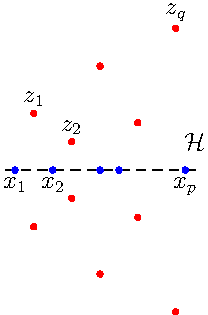
\includegraphics{C1622_1.pdf}
 \caption{Racines complexes d'un polynôme à coefficients réels}
 \label{fig:C1622_1}
\end{figure}

\begin{rem}
 On peut donc regrouper par deux les racines non réelles. Il est commode de repérer chaque couple par l'élément qui est dans le demi-plan $\mathcal H$ formé par les complexes de partie imaginaire strictement positive.
\end{rem}


\index{polynômes irréductibles de $\R[X]$}
\begin{prop}[Polynômes réels irréductibles]
Les polynômes irréductibles de $\R[X]$ sont les polynômes de degré $1$ et les polynômes de degré $2$ sans racine réelle.
\end{prop}
\begin{rem}
 Le polynome réel de degré 2 dont les racines sont des complexes non réels $z$ et $\overline{z}$ est
\begin{displaymath}
 (X-z)(X-\overline{z})=X^2 - 2\Re(z)X+|z|^2
\end{displaymath}
\end{rem}


\index{décomposition en facteurs irréductibles dans $\R[X]$}
\begin{prop}[Décomposition des polynômes réels en facteurs irréductibles réels]
 La décomposition en facteurs irréductibles d'un polynôme $P$ à coefficients réels est de la forme suivante.
\begin{displaymath}
 P = \lambda \prod_{k=1}^p(X-x_k)^{m_k}\prod_{k=1}^q(X^2 - 2\Re(z_k)X+|z_k|^2)^{n_k}
\end{displaymath}
où $\lambda\in \R$ est le coefficient dominant de $P$, où les $x_k$ sont les racines réelles de $P$ et $m_k$ la multiplicité de $x_k$, où les $z_k$ sont les racines de $P$ dans $\mathcal H$ et $n_k$ la multiplicité de $z_k$.
\end{prop}


\section{Formule d'interpolation de Lagrange}

\index{polynômes d'interpolation de Lagrange}

Soit $x_0,\cdots,x_n$ des éléments distincts de $\K$, on définit les polynômes $L_0,\cdots, L_n$ par :
\begin{displaymath}
 L_i = \prod_{j\in\llbracket 0 , n \rrbracket j\neq i}\frac{X-x_j}{x_i - x_j}.
\end{displaymath}
Par définition, ils sont de degré $n$ et vérifient
\begin{displaymath}
 \forall (i,j) \in \llbracket 0, n \rrbracket^2:\; \widetilde{L_i}(x_j) = \delta_{i,j}
=
\left\lbrace 
\begin{aligned}
 0 &\text{ si } i\neq j \\ 1 &\text{ si } i = j 
\end{aligned}
\right. 
\end{displaymath}
\index{symbole de Kronecker} $\delta_{i,j}$ est appelé le \emph{symbole de Kronecker}.
\begin{prop}
Soit $x_0,\cdots,x_n$ des éléments distincts de $\K$. Pour tout $n+1$-uplet $(y_0,\cdots,y_n)$ d'éléments de $\K$, il existe un unique polynôme $P$ de degré inférieur ou égal à $n$ tel que 
\begin{displaymath}
 \forall i \in \llbracket 0 , n\rrbracket,\; \widetilde{P}(x_i) = y_i
\end{displaymath}
Il s'exprime comme combinaison des $L_i$:
\begin{displaymath}
 P = \sum_{i=0}^n y_i L_i .
\end{displaymath} 
\end{prop}
\begin{demo}
 En utilisant le résultat relatifs aux valeurs des $\widetilde{L_i}(x_j)$, si 
\begin{displaymath}
 P = \sum_{i=0}^n y_i L_i
\end{displaymath}
on vérifie facilement que $\widetilde{P}(x_i) = y_i$ pour tous les couples $(i,j)$.\newline
Si $P$ et $Q$ sont deux polynômes vérifiant les conditions imposées, alors $P-Q$ est un polynôme de degré strictement plus petit que $n$ et qui admet les $n$ racines $x_0,\cdots,x_n$. C'est donc le polynôme nul ce qui assure l'unicité.
\end{demo}
\begin{rem}
 Plus généralement, si $Q$ vérifie $\widetilde{P}(x_i) = y_i$, alors tous les $x_i$ sont des racines de $Q-P$ qui est donc divisible par $(X-x_0)\cdots(X-x_n)$. On en déduit qu'il existe un polynôme $\Lambda$ tel que 
\begin{displaymath}
 Q = P + \Lambda (X-x_0)\cdots(X-x_n).
\end{displaymath}
\end{rem}
\end{document}
